\documentclass[a4paper,11pt]{kth-mag}

\usepackage[T1]{fontenc}
\usepackage{amsfonts}
\usepackage{textcomp}
\usepackage{graphicx}
\usepackage{hyperref}
\usepackage{lmodern}
\usepackage[utf8]{inputenc}
\usepackage[swedish,english]{babel}
\usepackage{nada-ex}
\usepackage{subcaption}
\usepackage[backend=biber]{biblatex}
\usepackage{csquotes}
\usepackage{tikz}

\def\arraystretch{1.5}

\addbibresource{ressources.bib}

\graphicspath{{img/}}

\title{Inside the Black Box: How to Explain Individual Predictions of a Machine Learning Model}
\subtitle{How to automatically generate insights on predictive model outputs, and gain 
	a better understanding on how the model predicts each individual data point.}
\author{Marc Beillevaire}
\date{December 2016}
\blurb{
	Master's Thesis at CSC \\
	Supervisor: Hedvig Kjellström \\
	Examiner: Danica Kragic
}
\trita{TRITA xxx yyyy-nn}
\begin{document}
\frontmatter
\maketitle


\begin{abstract}
Machine learning models are becoming more and more powerful and accurate, but their good predictions usually come with a high complexity. Depending on the situation, such a lack of interpretability can be an important and blocking issue. This is especially the case when trust is needed on the user side in order to take a decision based on the model prediction.

In this thesis, several explanation methods are described and compared on multiple datasets (text data, numerical), on classification and regression problems.
\end{abstract}

\clearpage
\selectlanguage{swedish}
\begin{abstract}
på svenska

jag tycker om kannelbullar
\end{abstract}
\selectlanguage{english}
\clearpage
\tableofcontents
\mainmatter



\chapter{Introduction}

This first chapter is an introduction to the problem raised in this master thesis and provides an overview on how it is structured. It first describes the backgrounds and motivations for this project, and set the research question as well as a high-level view on the methodology and the approach chosen to deal with it.

\section{Background}

This project has been conducted at \textit{Dataiku}, in Paris. Dataiku is a young startup developping \textit{Dataiku DSS} -- standing for Data Science Studio. This software is a collaborative plateform on which data scientists and data analysts can easily perform data processing operations, such as: collecting the data, cleaning it and doing some preprocessing, training and applying machine learning algorithms as well as putting a process into production in a few clics.

Besides developping Dataiku DSS, the company also helps companies to set up data science projects by providing both the technical solutions and the scientific expertise from Dataiku's data scientist team. Today, their customers are spread out around the world. After securing a series A fundraising in October 2016, the company's next goal is to appear among the top data science plateforms in the USA anytime soon.

This project was initiated after several feedbacks from Dataiku customers. They are always looking for more trust and transparence towards the models they are using, and this is one of the key issues when machine learning models are required for taking actions in a company. Thus, Dataiku's customers are often asking for more insights, and many of them especially want to know why such a prediction has been made by a given model, on a given data point.

This projects aims at providing a selection of practical solutions to this problem to the Dataiku team. The purpose is also to make their use simple by providing Dataiku DSS plugins, as well as webapps for visualization purposes.

\section{Motivation}

Predictive models using machine learning are getting more and more efficient while spreading in many areas in both industrial and services companies. Many companies are collecting and using their own data more and more to optimize various processes. For instance, in online marketplaces customers' data are constantly processed by machine learning algorithms, whether it is for recommendation or to track potential fraudsters.

Yet, while most companies are eager to set up very efficient predictive models, a strong limitation still holds: when a human decision maker has to take an action \textit{according to a prediction made by a model}, trust in the model becomes at least as important as the accuracy of the prediction itself. People cannot willingly accept to take a decision just because a computer said so, and they need to be provided with insights and explanations on why the model produced a given output. This is why the demand for new insights at the prediction level is important: global coefficients at the model level are not enough, most of the time the real question is \textit{"Why this model made such a prediction ?"}.

This is the case in many areas: in fraud detection on an e-commerce website,  taking an action could mean adding another layer of security during a purchase like 3D security, which decreases the user experience and could lead to fewer purchases. With predictive maintenance models, maintenance operations on the equipment costs money, and such a predictive model would be used by decision makers \textit{only} if they believe the algorithm can effectively predict the next failures of the equipment. Hence how efficient such models may be, they would only be applied if the business owners trusts them to effectively optimize the company's processes.

This necessity for insights is going to be more significant in the years to come in the European Union. Indeed in April 2016, the European Parliament adopted \href{http://eur-lex.europa.eu/eli/reg/2016/679/oj}{the General Data Protection Regulation (GDPR)}. Besides new rules regarding data protection, it provides every European citizen a \textit{right to explanation} \cite{euregulation}: every decision having an impact on someone's life will have to be motivated by an explanation, even when the decision is taken by an algorithm. For instance, a bank agency will not be able to refuse a loan based only on an algorithmic decision.

\section{What information should an explanation bring ?}
% Titre ok ??

The main purpose of individual explanations is to bring \textit{trust} to users of machine learning models. According to some articles, interpretability is a prerequisite for \textit{trust} \cite{lime} \cite{mythos}. Trust could actually be assessed by a simple score of the model, but it usually requires more than that: users are generally more comfortable when they understand the models they trained. Moreover, one can trust a model to be efficient, but not to respect some criteria and constrainsts such as ethics or legality \cite{mythos}.

Therefore, an explanation algorithm must ensure understandability in each predictions that are explained. This mean producing an output that is easy to read and interpret for a human being, and that relies on the users' previous knowledge on the data in order to help them understand the model's behaviour.

This leads to the following remarks: an explanation should be kept short, so that it is immediately fully understood by the user. For instance: a linear model, even easily interpretable by nature, will not be understood if there are several hundreds of variables. Besides, the user is supposed to have knowledge on the features in the dataset, so it is fine to use this in order to build explanations.

Therefore, in this thesis an explanation will consist on a short list of features, with a weight assigned to each of them.

\section{Problem statement and methodology}

The goal of this thesis is to test several algorithms that automatically extract explanations from the model and to assess their goodness to compare them.

These algorithms have two main purposes: effectively provide explanation for each prediction made by the model, and also assessing the goodness of the model. Indeed when looking at explanations, a user with prior knowledge on the data will be able to tell if the model relies on relevant features. If a model is trained and tested on a datasets where some features are falsly correlated to the output, then the model is probably not very good -- not generalizable on new data that does not provide these falsly correlated features.

For instance, assume an image classification model only sees the blue sky to detect airplanes. If there are only planes in the sky, its score will probably be high. But what if a bird flying in the sky is set as input ? The model has a high probability to classify it as a plane.

Using efficient explanations, this could be anticipated: the explanations for examples in the \textit{plane} class would show that only the blue sky matters to the model. Human beings can clearly see that the model did not detect the real object. Therefore they could assess that this model is not actually good at classifying planes, no matter how high its accuracy on the test set is.

In this project, this goodness measure will be used to test the explanations algorithm. The goal of the explanaining algorithm is to point out the wrong features that are used by bad models. So our methodology will be the following:

\begin{itemize}
	\item Set up two datasets: one with both useful and useless features, another one containing only the good features
	\item Train a model using the first dataset, test it on the second one
	\item Extract explanations from predictions on several examples
	\item Remove the bad features that popped up in the explanations, retrain the model
	\item Check if the score improved on the second model
\end{itemize}

Here, we expect the score on the second dataset to be quite low, because the model learned some wrong correlations between useless features and the target. If the explanations are relevant, they should point out the most important features that are used by the model on several examples. Using the prior knowledge on the features, the bad ones can be removed, and the score on the second (clean) set should improve.

\section{Framework}

Most of the time explanations algorithms can work with any type of model: either regression or classification models as long as they output probability for each class. We will focus on classic, widely-used algorithms such as linear models, Classification and regression trees \cite{cart}, Random Forests \cite{Breiman2001}, Gradient Boosted Trees \cite{Friedman2001}.

The type of data that will be considered will be tabular data sets (feature vectors with a target) as well as textual data. This is of course generalizable to any type of data, like image classification and neural networks, but to stick with reasonable amount of data and limited training time, these kind of datasets and methods will not be investigated.

The method will be tested on several datasets. Therefore the output will be changing, and an algorithm can be good to extract explanations on specific data while being less efficient on other datasets. Yet, we expect our methodology to show consistent results that should not vary too much between different datasets.

\section{Outline}

This thesis is divided into 5 chapters.

The \textit{Introduction} chapter provides the background and motivation for this project. The methodology is also stated, as well as the hypothesis for an explanation algorithm to be good enough. Finally the framework part provide information on the frame and the limitations of this thesis.

The \textit{Background} chapter focuses on the algorithms published in the litterature, where the most important papers in this field of research will be examined. This chapter will also cover the background knowledge needed for the rest of the thesis. Not so many papers are related to model explanations at the prediction level. Yet they nearly all propose a different approach to this issue.

The \textit{Method} chapter is dedicated to how the experiment will be performed. The datasets are specified, as well as the various models used for the tests. The technical content will be further described in this chapter. Especially, several algorithms that compute explanations on individual predictions will be provided. The metrics used to assess whether an algorithm is good or not to extract explanations is also further described here.

The \textit{Experiments} part describes the experiments conducted in this thesis. This chapter provides all the results obtained according to the method of the previous chapter.

Finally, the \textit{Discussions} chapter summarize the results and discuss the different methods explored here. This chapter also describe some limitations to this thesis, and provides potential improvements and what could be the future work on this topic.

\chapter{Background}

This chapter provides the technical background to this thesis. The litterature study show a relatively important interest in this field for the last decade, and a great variety of algorithms presented in research papers.

This chapter is divided in two parts as there are two main solutions for this problem of explaining individual models' predictions. Either the algorithm uses the inherant structure of the model to compute explanations like the tree structure for tree-based models. Or it considers the model as a black box and only uses the input-output matching that it produces.

The first type of algorithms will be called \textit{model-dependent} explanations algorithms, while the second type are denoted by either the term \textit{model-independant} or \textit{model-agnostic} explanations. Both these two solution have some advantages and drawbacks, and several implementations in these two categories will be investigated.

\section{Model-dependant explanations}

This first type of explanations implies for the explanations algorithm to understand how the explained model is build, making use of its particular type to extract explanations from it. A real advantage for these methods is that explanations are usually faster to compute. Yet, they suffer from not being generalizable to other types of models. Moreover two different model-dependent explanations cannot be compared if they has been computed on two different types of models.

\subsection{Linear models}

By definition linear models are easy to interpret without a complicated on-top explanations algorithm: one only has to look at the regression coefficients to see the relative importance of each variable.

The output of a linear model is the following:

\[
	P(x_1, ..., x_n) = f \left( \sum b_i x_i \right)
\]

where $(x_1, ..., x_n)$ is the current data point, and the values $(b_i)_{i \in [1, n]}$ are the coefficients of the linear model. The function $f$ maps the sum into the output space. For linear regression, $f$ is the identity function, while for logistic regression, $f$ is the sigmoid function: $f(x) = \frac1{1 + e^{-x}}$.

It is then easy to compute the contribution of the features to the outcome: as the output depends directly on the sum of the feature value multiplied by the regression coefficient, multiplying each regression coefficient by the feature value give the direct influence of the feature value on the prediction. Each term $b_i x_i$ represents therefore the influence of each feature to the output. In the case of linear regression, it is even the direct contribution to the output, but for logistic regression, the sigmoid function prevent from a meaningful comparison between each $b_i x_i$ and the predicted value.

\begin{center}
	[ Insert picture maybe ?]
\end{center}

The limit in interpretability of a linear model is only the dimension of the input space: if there are hundreds of features to consider, then another step is needed. It can simply be a list of the top $N$ coefficients, $N$ being small enough. But we could also consider a feature selection algorithm that keeps a small number of features before fitting the model.

The interesting thing in linear models is the ability to predict how the model will behave when moving the data point in the feature space. It only requires to look at the model coefficients: a positive coefficient means that increasing the feature increases the output, and vice-versa with negative coefficients. For interpretation purposes, this is very convenient: when users of a model can take actions to change the input variables, they know which ones to change in order to adapt the output.

\subsection{Tree-based models}

An explaining algorithm for tree-based models -- classification and regression trees, random forests and gradient boosted trees -- has been developed by \citeauthor{treeinterpreter} in a blogpost \cite{treeinterpreter}.


It works as follow: initially the contribution for each feature is set to 0. When computing predictions using a tree, the data point $x$ goes down in the tree, starting from the root, following a series of rules based on the features values. At each step down, the features space is split into two disjoint parts along one axis because only one feature is involved in one cut. The algorithm then computes for this cut the difference between the proportion of $\hat{y}$ -- the model output -- in the subspace where $x$ lies and the proportion of $\hat{y}$ in the bigger space.

This quantity is summed to the contribution of the feature involved in the cut. This value answers the question: at a given step, how well did the feature improve the classification of the example ?

To understand this process better, let's assume we have a train dataset of 2-dimentional points, a new example to classify, and that we use the following tree to classify the points into two classes:


\begin{figure}[h!]
\centering
\begin{subfigure}{.55\textwidth}
	\centering

	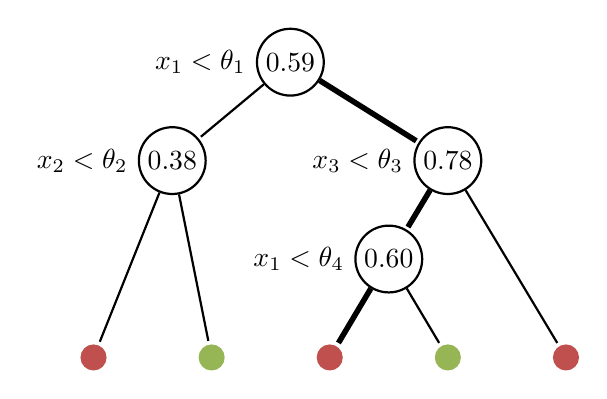
\begin{tikzpicture}[->,>=,shorten >=1pt,auto,thick,
    	 inner node/.style={circle,draw,inner sep=2pt},
    	 red node/.style={circle,fill=pastelred},
    	 green node/.style={circle,fill=pastelgreen}]

	\definecolor{pastelred}{RGB}{192,80,77}
	\definecolor{pastelgreen}{RGB}{150,182,86}

  	\draw (0,0)     node[inner node,label=left:$x_1 < \theta_1$] (1) {0.59};
	\draw (-1.5,-1.25) node[inner node,label=left:$x_2 < \theta_2$] (2) {0.38};
	\draw (2,-1.25)  node[inner node,label=left:$x_3 < \theta_3$] (3) {0.78};
	\draw (1.25,-2.5)    node[inner node,label=left:$x_1 < \theta_4$] (4) {0.60};
	
	\fill (-2.5,-3.75)   node[red node]   (5) {};
	\fill (-1,-3.75) node[green node] (6) {};
	\fill (0.5,-3.75)    node[red node]   (7) {};
	\fill (2,-3.75)  node[green node] (8) {};
	\fill (3.5,-3.75)    node[red node]   (9) {};
  	
  	\path[every node/.style={font=\sffamily\small}]
    (1) edge      (2) 
        edge[line width=2pt] (3)
    (2) edge      (5)
        edge      (6)
    (3) edge[line width=2pt] (4)
        edge      (9)
    (4) edge[line width=2pt] (7)
        edge      (8);
        
	\end{tikzpicture}
  
  \caption{A subfigure}
  \label{fig:sub1}
\end{subfigure}%
\begin{subfigure}{0.45\textwidth}
  \centering
  \includegraphics[width=1.0\linewidth]{img/decisiontree.png}
  \caption{A subfigure}
  \label{fig:sub2}
\end{subfigure}
\caption{A figure with two subfigures}
\label{fig:test}
\end{figure}

The green and red dots represent the training set, and the grey dot a new example to classify. At each node of the tree, a test is performed (Is $x_i$ smaller than $\theta_j$ ?) in order to drive the grey point either on the left or the right branch. The numbers on the nodes indicate the proportion of red dots in each subspace represented by this node. On the leafs, this proportion is either 0 or 100\% -- the leaf represents either a green subspace or a red subspace here.

The grey dot is the new example to classify. It will, of course, be classified as red by the classification tree, going through the bold path to the red leaf. 
Between the root and the second node encountered by the example while being classified, the feature $x_1$ is used, and the classification improves since the proportion of red points goes from 0.59 to 0.78. Hence, the contribution of feature $x_1$ is positive at this step and is increased by $0.78 - 0.59 = 0.19$.

Then feature $x_2$ is used, and this step reduces the proportion of red dots by $0.18$. Finally, feature $x_1$ is used again, increasing the probability from 0.60 to 1. 

Summing all the contributions along the path, the explanation for this classification are the following contributions towards class \textit{Red}:

\begin{center}
\begin{tabular}{|c|c|}
\hline
Feature $x_1$ & 0.59 \\
\hline
Feature $x_2$ & -0.18 \\
\hline
\end{tabular}
\end{center}

This solution is easily adaptable to ensemble methods using trees as their base model: contributions to each feature can be summed over all the trees, and average according to the importance of each tree in the classifier.

In the case of Random Forests, where all the trees are given the same weight, contribution for feature $i$ is computed as follow:
\[
	\mathrm{contrib}_i(x) = \sum_{tree t} \mathrm{contrib}_{t,i} (x)
\]

This way of exploring trees through the path of the original datapoint makes this algorithm efficient: its complexity is proportional to the height of the tree, and linear in the number of trees if the algorithm is an ensemble.

\section{Model-independent explanations}

Although model-dependent methods are computationally efficient, they still rely on specific models. A model-independent or model-agnostic algorithm would be preferable for at least two reasons: its ability to explain any type of classifiers and regressors, and the possibility to compare two explanations from two different model, even when these models are of different types.

Several algorithms has been developed, most notably: \cite{lime}, \cite{explvect}, \cite{ice}, \cite{gametheory}, \cite{documentclassif}. They nearly all develop a different approach to extract explanations from a specific prediction, albeit some similarities exist between some of them.

For some authors, the way to understand a prediction is to locally estimate the output of the model. That is, understand how the model behave around the data point of interest in the features space.

Thus, several solutions involve estimating the local output distribution from the model, like \textit{Lime} \cite{lime} and \citeauthor{explvect}'s \textit{explanation vectors} \cite{explvect}. If the model is a classifier that outputs probabilities, then the output distribution is a probability distribution in the feature space. 

\subsection{Local estimation by a simpler model}

\textit{Lime} algorithm \cite{lime}, standing for \textit{Locally Interpretable Model-agnostic Explanations}, is a recent solution proposed by \citeauthor{lime}. The authors' main idea is to locally estimate a complicated model by a simpler one that is interpretable. The goal is then to find a new model that is a good local estimator of the complex model, so the new model should be locally faithful to the original model.

Given the constrainst of interpretability, linear models are the first obvious choice to use as simple models. When a limited number of features is used, then such models become easily interpretable by humans. Simple decision trees that are not too deep could also make good interpretable models, but only linear models will be used here.

To locally approximate a model seen as a black box by a linear model, Lime's process is the following:

\begin{itemize}
	\item Sample $N$ points according the the training set distribution. Generally several thousands of points are needed so that Lime gets an accurate enough view of the training set.
	\item Apply the black box estimator to each of the sample. All these outputs will form the targets of the new training dataset.
	\item Weight each sample using a gaussian kernel centered on the point of interest
	\item Fit a linear model to the new dataset formed by the samples and the complicated model outputs.
\end{itemize}

\begin{figure}[!h]
	\centering
   	\def\svgwidth{\columnwidth}
	\includegraphics{lime-schema.png}
    \caption{Local estimation by a linear model around the bold red cross}
\end{figure}

In the author's implementation \cite{limeGitHub}, the sampling is made after \textit{discretizing the training set}: each feature is splitted in several parts using a binning method (quantiles, histograms, supervized binning). Then each new sample is generated feature by feature following this binning. This may not be the most accurate way to mimic the training distribution but it is quite fast --- linear in the number of features. Furthermore, the goal is only to generate points in space, and the fact that some of them are distant from the initial point is not a problem since the gaussian kernel weighting (at step 3) will keep the linear model locally accurate: points that are far away will not be taken into account in the local model, while closer ones will be considered as most important.

Finally, the interpretation of the simple model is the easy part: it only requires to check the features associated to the biggest coefficients of the linear model. These biggest coefficient actually represent the locally most effective features that had the most importance on the prediction since variations on these features whould have led to the larger changes on the model output.

\subsection{Gradient of the model output distribution}

\citeauthor{explvect}'s \textit{explanation vectors} algorithm \cite{explvect} have a comparable approach to Lime's, in the sense that they both try to mimic the local distribution.

The model output is here estimated using a non parametric estimator around the point of interest. Then the gradient of this estimator at the inital point is computed. The largest absolute values of the gradient components are the most locally influential variables on the prediction, for the same reason as in Lime algorithm: along these features, local small variations would mean large variations of the model output.

The main issue here is to estimate the probability density of the classifier output. The authors adress it using the Parzen-Rosenblatt window method \cite{parzen} \cite{rosenblatt}: a density estimation method that interpolates several points with a sum of kernels. Practically, this means sampling in the dataset, and adding to the sum a new kernel for each new sample. At each step, the estimated distribution is the following:

\[
	P(x) = \frac{1}{n} \sum_{i=1}^n \frac1{h_n^d} K \left( \frac{x - x_i}{h_n} \right)
\]

where $K$ is a $d$-dimentional kernel function, $(x_i)_{i \in [1,n]}$ are the $n$ samples and $h_n$ is the bandwidth of the kernel, usually depending of the number of samples drawn. The most widely used kernel function is the Gaussian kernel. It is convenient here, being differentiable, and once the density is well-estimated by the window, computing the gradient from a sum of gaussian functions is very straightforward.

\subsection{Explanations through visualization}

Visualizing is key to understand how datasets are structured, especially with the large amount of new data that appears everyday. This is why easily understandable explanations should be mixed with visualization tools.

Nevertheless, as opposed to the previouly mentionned algorithms, another class of explanations uses visualization as the central part of the process. It regroups methods like Partial Dependence Plots (see \cite{elementsofstats}), and Individual Conditional Expectation \cite{ice}.

The principle of Partial Dependence Plots is to show on a graph how the model output evolves when a single feature is changed, that is: given an estimator $f$, a point in the features space $\mathbf{x} = (x_1, ..., x_n)$ and a feature $i$, computing the following function:

\[
	f_i : x_i \mapsto \mathbb{E}_{x_i} (f(\mathbf{x})) = \int f(x_1, ..., x_n) \mathrm{dP}(\mathbf{x}_{(\neq i)})
\]

where $\mathbf{x}_{\neq i} = (x_1, ..., x_{i-1}, x_{i+1}, ..., x_n)$

Usually the expectation above is computed through the following sum:

\[
	f_i(x_i) = \sum_{i=1}^{N} f(x_1,... , x_n)
\]

When plotting this function, the user can have an idea how \textit{in average} the model would evolve when changing the variable $x_i$.

The Individual Conditional Expectation plots idea is that averaging in such a way the estimator over the other variables reduces the information provided by the plot, and that it sometimes doesn't help the user understand the data.

Therefore, instead of computing the expectation value over all the examples, ICE's authors decide to keep one curve for each instance.Then for each feature $i$ and example $k$, the following functions are plotted on the same graph:

\[
	f_{i,k}(x) = f(x_1, ..., x_{i-1}, x, x_{i+1}, ..., x_n)
\]

This lets the user having far more insights on the model behaviour on individual instances, without being longer to compute than a partial dependence plot. Of course the graph should be kept readable and a limited number of lines should be plotted. The authors also proposes to "pinch" all these plots on one location $x^*$ in the range of $x_i$, thus ploting the centered ICE plots, the \textit{c-ICE}:

\[
	f^\mathrm{cent}_{i,k}(x) = f_{i,k}(x) - f(x_1, ... x_{i-1}, x^*, x_{i+1}, ..., x_n)
\]

as well as drawing the derivative of all these plots (the \textit{d-ICE}) to understand better where important interaction happen for this feature.

\subsection{Explanations using Game Theory}

A final interesting approach relies on game theory and the \textit{Shapley value} to compute explanations \cite{gametheory}.

The Shapley value was first introduced by Lloyd Shapley in 1953 \cite{shapleyvalue}. It can be described as an "a priori evaluation of the prospects of a player in a multi-person game" \cite{hart1989shapley}. The Shapley value represents therefore the influence of a player regarding potential coalitions formed with other players. For instance in the Council of the European Union, each country has a number of votes proportional to its population: bigger countries have a more votes and can make stronger coalitions, while smaller ones have less. The Shapley value in this EU Council reflects this power: Germany and France have a larger Shapley Value, while less populated countries have a small Shapley Value. 

In this article \cite{gametheory}, the "players" in the game are the input variables of the model. They "compete" in a certain way to influence the model output. Therefore, the features that had the most importance in a specific prediction should get a larger Shapley value.

The real challenge is to compute the Shapley Value, which is hard in practise, due to an exponential computationnal time. The authors show that the Shapley value of feature $i$ can be written in the following way:

\[
	\varphi_i = \frac1{n! \, . \, | \mathcal{A} |} \sum_{\mathcal{O} \in \pi(N)} \sum_{y \in \mathcal{A}} \left( f( \mathrm{Pre}^i(\mathcal{O}) \cup \{i\}, y) - f(\mathrm{Pre}^i(\mathcal{O}), y) \right)
\]

where $\pi(N)$ is the set of permutations of all the features, $\mathcal{A}$ is the feature space. $\mathrm{Pre}^i$ represent here all the features before feature $i$ in the permutation $\mathcal{O}$. This sum can be approximized by sampling datapoints in $\mathcal{A}$ and premutations $\mathcal{O}$ of the features.

Yet, with a large number of features, the number of samples required to estimate the Shapley value increases a lot. Consequently convergence time become too important for most use cases.

\subsection{Explanations on textual data}

Textual data is quite different from classical data like churn prediction, or fraud detection datasets: the data is less structured, and variables are usually words or group of words. This leads to a very high dimentionality for large corpuses. Other explanations methods may not work as efficiently here.

Two articles focus on explaining classification of text documents: \citetitle{documentclassif} \cite{documentclassif}, and also part of the Lime article \cite{lime}.

The first one (\cite{documentclassif}) intend to find the \textit{minimal explanation} in a document classification. This minimal explanation is the smallest set of words in a document that changes the classification result of this document. That is: a set $S = \{w_1, ..., w_k\}$ where removing all the words $w_1, ..., w_k$ from the document changes the classification, while removing only part of this set does not.

The classification explanation is then the previous set of words. Yet finding large sets of words in documents leads to a large complexity (exponential complexity). The authors therefore propose an heuristics to find these sets: first find words that changes the most the output probability, then combine these strong words together in order to find the minimal explanation. The complexity for this second solution keeps polynomial.

\vspace{\baselineskip}

Lime \cite{lime} also features a specific part on explaining text classification.

The solution uses Lime algorithm -- described above -- adapted to this kind of data. Here instead of sampling data in a classical features space, new documents are sampled by randomly removing words from the original document. Distances between the new texts and the initial document are measured using cosine distance.

Then, Lime is applied: the samples are weighted using a distance kernel centered in the original document, and a linear model is fitted. This method is quite efficient and not too expensive, as the complexity is linear in the number of samples chosen.

\chapter{Method}

The purpuse of this thesis is to test which algorithms provide the most meaningful explanations, and which explanations are the most significant in order to get insights on a classifier and to improve it.

This chapter first provide some information on explanations and present the main difference between two kind of explanations. Then the method for measuring the score and ranking the algorithms is provided.

\section{What an explanation means in practise}

An explanation is a set of features that are given a weight, but what this set means can be seen in two ways. Each has its advantages and its application purposes, and they do not necessarily lead to the same results.

\subsection{Contribution to the output value}

First, the influence of the features can be defined as their contribution to the prediction, such that summing all the influences gives back the actual prediction. Here by prediction, we mean \textit{probability} for classification or \textit{raw value} that the model predict for regression. This methods involves splitting the prediction into several part, then associating to the influential features the biggest parts and to the less influential the smallest.

For instance, let us consider a binary classification model for the Titanic dataset, that assess the probability between 0 and 1 that the person survives.
If for a given individual, the prediction is 80\% chances of survival, then the explanation could tell us that:

\begin{itemize}
\item being a woman, her survival probability increased by 32\%
\item being a first class passenger, it also increased by 15\%.
\item but being 47 years old, the probability of survival decreased by 3\%
\end{itemize}

This kind of explanation is described on figure 1.1. Here the model attempts to predict whether passengers from the Titanic have survived or not. It is based on a random forest with 250 trees, so examining all the trees to try to understand a single prediction is totally intractable for a human being.

In average, in the dataset, a passenger has an probability of survival equal to $0.38$. But for this example the model predicts survival with probability $0.93$ which is $0.55$ higher than the average value. This difference of $0.55$ is then due to the feature values of this particular example. Using this type of explanation, we can actually compute this difference, and moreover know how each feature influenced it. 

\begin{figure}[h!]
		\centering
    	\def\svgwidth{\columnwidth}
    	\input{img/1-2-2.pdf_tex}
    	\caption{Summing all the influences starting from the average probability}
    \caption{Classification model on the Titanic dataset, explanation for one passenger: a women, travelling in the first class, with a high ticket fare. This type of explanation enables summing all the feature influences, starting from the average probability to reach the classifier's prediction.}
\end{figure}

Figure 1.1 provides the influences for each feature. Chart (a) is the raw influence in terms of probability. On figure (b), each step corresponds to the increase produced by each feature value. With this kind of plot, one can easily concludes that \textit{Sex} is the most influent feature, since given all the other features, it increases the probability from around 0.62 to 0.95.

This way of building explanations produces very clear and understandable explanations. Indeed, it is easy to understand that here the \textit{age} feature has a negative contribution to the output probability of survival -- people in their fourties rather died than were saved, while the \textit{Pclass} feature has a positive impact -- only a few first class passengers died. Besides, it is easy to limit the set of important features by taking only the first $N$ relevant, and summing the rest of the influences into an additional \textit{"other features"} category.

Nevertheless, these types of explanations have one drawback: even if for a single point it gives clear and understandable explanations, we have no idea of what happens when this point shifts a bit in the features space.

For instance we could be intereseted in knowing what happens when a given feature increases or deacreases. For a pricing prediction model, knowing which feature to change to increase the revenue is much more important than the actual output contribution.

\subsection{How the output changes}

As stated before, more than the contributions of each variable, we would like to know how the classifier behaves when our point of interest shifts a bit in the feature space.

This would allow the user to know how to change the variables in order to change the input. For instance, managers of a production line are provided with a predictive maintenance model. But instead of knowing which parts are likely to break, they would be interested in knowing how to reduce the breaks and the maintenance costs. So the important question for them would be: which important variables should be changed to reduce the costs. Therefore, using such an explanation answering this question, they could adapt the production line  according to it by changing the variables in a way such that the model would predict less maintenance cost, or a longer lifetime.

Building such explanations actually means having an idea of how the outcome changes when moving around the initial point, and therefore this means estimating the outcome around this point. As our models here produce probabilistic outputs, the outcome is here a probability distribution.

These kinds of explanations should give insight about how the distribution evolve, and point out which features to change to get the expected output.


\section{Performance measure}

In this problem of finding explanations of individual predictions, the output cannot be evaluated as simply as an accuracy score. The output is here a list of variables along with a weighting score, and it is therefore much more qualitative than quantitative. Moreover an explanation algorithm can be helpful on a given dataset and not on another, but performance can also vary from an individual example to another one.

Hence the measure of the performance of an algorithm will not be based directly on the algorithm output, but rather on its ability to help humans in understand and improve a model.

The performance test for an algorithm will be the following: first a bad model will be trained on a given dataset. A \textit{bad model} is a model based on features that the user know not to be reliable. Then explanations are computed for several examples in the test dataset. A user is then asked to remove the features that does not seem trustworthy.

To test the algorithm quantitatively, two datasets are needed apart from the training set: one test dataset in the same format as the train set, that is, not cleaned from the untrustworthy features, and a validation dataset that contains only the clean data.

That way, the baseline score of the model is the score on the validation set: this is the score the model would obtain when applied on external data, it shows the ability for the model to generalize or not on new data. Meanwhile, the score on the unclean test set does not reflect the real performance of the model: this score should be probably higher than the one on the clean validation set. The higher the difference between these two score, the less trustworthy and generalizable the model is.

When the untrustworthy features are identified by the user, these features are removed from the original set -- the train and test datasets. Then a new model is retrained and scored, both on the test set and on the clean validation set. The score on the test set may decrease, but it should get closer to the score on the validation set. Indeed, the algorithm is now supposed to be based on more trustworthy features, and the score on the test set should reflect more precisely the ability of the model to generalize on new data.

\section{Machine learning models}

The purpose of this thesis is to find and test several algorithms that would have practical use at Dataiku and in the industry in general. This is why popular models will be tested: models that are widely used in production in many datascience projects.

Therefore four models will be tested, two linear models: \textit{linear regression} and \textit{logistic regression}, and two tree-based models: \textit{Random Forests} \cite{Breiman2001} and \textit{Gradient Boosting} \cite{Friedman2001}. Nonetheless, regarding model-independant explanations, any type of predictive model could be used, as long as it outputs either classification probability, or a regression prediction, like neural networks for instance.

To measure the performance of the machine learning models, the Receiver Operating Characteristic (ROC) is used.

\section{Algorithms tested}

As seen on Chapter 3 -- Background, this field of research led to many different algorithms that intend to explain machine learning models. In this thesis, a selection of algorithms will be tested, with several variants.

\subsection{Model-dependant}

As we will use either linear or tree-based models here, two kinds of model-dependant explanations will be used.

For linear models, the simple explanation algorithm relying on the linear coefficients and the features value, presented in Chapter 3, will be applied. This solution works in a similar way for regression and classification, so it will not need any adjustments for linear regression or logistic regression.

When testing tree-based models, Tree Interpreter \cite{treeinterpreter}, implemente by the article author on github will be used for Random Forests. An adaptation for gradient boosting made by the author of this thesis will also be used.

\subsection{Model-independent}

Among the large choice of model-independent explanations algorithms, two of them will be tested: \textit{Lime} \cite{lime}, and the Parzen-window-based \textit{explanation vectors} \cite{explvect}.

These algorithms are the most recent and above all: the fastest regarding computation time. Computing explanations for an individual example should be something fast enough: a user does certainly not want to wait 2 minutes to get an insight about an \textit{single} prediction, a few seconds is a maximum. Moreover, a high computation time makes it much harder to compute explanations for a large number of examples.

\section{Datasets}

The various methods will be tested on several datasets.

The regression dataset that will be used here is the House Market Dataset in Ames, Iowa. The target is the house prices and the dataset contains 80 attributes, such as the size of the land, the area of the house, the neighborhood, or even the type of fence around the property. The main interest of this dataset is the number of features, compared to the classical Boston Housing dataset. It should therefore be much more representative of the common data found in practical problems today, where datasets featuring around one hundred features is very common.

The method will also be tested on part of the 20 News Group Dataset. This dataset is interesting for several reasons: it is textual data, meaning the dimensionnality is high. Moreover, the data is very noisy: the data are e-mails, with their headers and previous messages embedded. Therefore, it is very likely that a classifier would rely on wrong features such as words in the headers, or e-mail addresses and not the actual text.

Finally for classical classification, the German Credit dataset from UCI will be used.


\chapter{Experiments}

\section{Titanic dataset}

The firsts experiments will be performed on the well-known Titanic dataset. This dataset consists on the list of the Titanic passengers with several information provided on them. The train set contains the information about the person having died in the tragedy or not, and the goal of the model is to predict the chances of survival for people on the test dataset.

Here we will be using a subset of the features: the passenger's age, sex and class, in which port he or she embarked, the ticket fare, and the number of parents or children spouses or siblings aboard, which makes a total of seven features.

This first experiment comparison between several explanation models will be performed by presenting to the human user the predictions from two models and their explanations. Among the models, one is performing very well while the other has a lower performance. Explanations regarding the better model should make more sense to the user. Explanations on wrong predictions from the second model should on the other hand be meaningless: an explanation telling the user that a passenger of the Titanic died because she was a lady from the first class should be a sign that the model doesn't extract meaningful information. Indeed, being a woman and a first class passenger on the titanic greatly increases the chances of survival.

The best model is a random forest with 250 trees. Its ROC AUC is 0.96, which is very high. The bad model is built upon the first one by randomly changing the predicted probabilities of the first model. The second model's predictions is drawn from a normal distribution, centered on the first model's predictions, with a standard deviation of 0.3. This lowers the AUC to 0.80.

The user is provided with 20 examples from the test dataset, and must pick the best one according to the explanations of the predictions on these 20 examples.


***** RESULTS: on average, the users have 0.90 chance to pick the right with treeinterpretor / lime quartiles / lime entropy discretizer / explanation vectors, etc... *****

***** Presentation of the explanations for one particular example, one where Lime is good and expl vectors is bad. *****

\subsection{Lime}

\subsection{Treeinterpreter}

\subsection{Explanation vectors}



\section{20 news group}

As stated in the methodology part, to assess the performance of an explanation algorithm, we will try to check if it manages to improve a bad algorithm. This means relying on the user's previous knowledge on the data.

A good way to build a bad model is to train it over bad data. The 20 news group dataset is perfect for that, as it is very noisy. It consists on a series of messages on various topics. The noise comes from the presence of the email headers such as:

\footnotesize
\begin{verbatim}
	From: lerxst@wam.umd.edu (where's my thing)
	Subject: WHAT car is this!?
	Nntp-Posting-Host: rac3.wam.umd.edu
	Organization: University of Maryland, College Park
	Lines: 15
\end{verbatim}
\normalsize

Moreover, there are quotations from previous messages, which can also worsen the classifier's performances.

In this experiments, we will only keep subsets of the 20 news group dataset consisting of the classes \textit{alt.atheism} and \textit{soc.religion.christian}. The goal of the classifier is to determine whether the document was about atheism or religion.

To build the initial classifier, the process will be the following: compute the \textit{Term Frequencies-Inverse Document Frequencies} (Tf-Idf) of the corpus, and train a machine learning algorithm on the Tf-Idf. Then the user observes a series of examples and their explanations. The bad features that show up in the explanations, such as words from the header, are removed, Tf-Idf is recomputed and a new model is trained.

The ROC curves that are obtained when scoring the model on the test dataset and the clean validation dataset are plotted on figure 4.2.

\begin{figure}[h]
		\centering
    	\def\svgwidth{\columnwidth}
    	\resizebox{0.75\textwidth}{!}{\input{img/roc-1.pdf_tex}}
    	\caption{Roc curve on the noisy test dataset (\textit{blue}, Area under curve: 0.986) and on the clean validation set (\textit{green}, AUC: 0.880)}
\end{figure}

As expected, there is a large difference between the score on the test set, that features the headers and previous messages quotations, and the validation set, cleaned from these noisy parts. These ROC curves mean that the model generalize badly on a clean dataset that is quite different from the training set.

Below are the results for the three kinds of explanations algorithms tested. The user is showed 20 examples from the dataset. These examples are the same in the three methods.

\subsection{Treeinterpreter}

\subsection{Lime}

Lime outputs the following dashboard, featuring the score of the model on this example, the words importance, and the text with important words highlighted.

\begin{figure}[!h]
	\centering
   	\def\svgwidth{\columnwidth}
	\includegraphics[scale=0.35]{lime-output.png}
    \caption{Example of output by Lime}
\end{figure}

According to Lime, the classifier clearly used several non-accurate words to classify this example, header words: \textit{Subject}, \textit{In article}, names: \textit{James}, \textit{Bill}, or just stop-words like \textit{you}, \textit{isn't}.

After a user is asked to watch a list of 20 examples and remove all the non-relevant words, the following list of word is build, to be removed from the original documents:

\begin{center}
\begin{verbatim}
saturn.wwc vice.ICO Beauchaine rutgers.edu .edu sgi Re
solntze edu Nntp Posting nih.gov writes rice.edu PSUVM re
athos.rutgers.edu Host bobbe@ Dwyer bil@ .com article
Distribution geneva.rutgers 1993 UUCP NNTP uk cmu umd.edu
okcforum Institute of Technology wrote
\end{verbatim}
\end{center}

Stop-words (\textit{the}, \textit{is}, \textit{a}, ...) are actually kept since they are also in the validation dataset. Words that are removed are words on which the original model relies, while being either on the header or any non-relevant part of the message.

When removing these words from the original dataset, the new model reaches the following scores:

\begin{figure}[h]
		\centering
    	\def\svgwidth{\columnwidth}
    	\resizebox{0.75\textwidth}{!}{\input{img/roc-2.pdf_tex}}
    	\caption{Roc curve on the noisy test dataset (\textit{blue}, AUC: 0.945) and on the clean validation set (\textit{green}, AUC: 0.902)}
\end{figure}

Of course the score on the test set decreases, as the number of features that are both in the train and test sets decreases.

But what is to be noted is the increase of the score on the validation set. This means that the models relies more on meaningful terms than before. Moreover, the two score get closer: the high AUC on the test set was misleading before, as there were many correlations between the target and non meaningful terms.


\subsection{Explanation vectors}

\vspace{5.0\baselineskip}

\begin{itemize}
	\item First train model on bad text
	\item Print expl with Tree Interpreter / Parzen / Lime
	\item Retrain 3 models, check the best ones
\end{itemize}


Also needed:

\begin{itemize}
	\item Check several bandwidths for Parzen \& Lime
	\item Check several binning algos for Lime
	\item Use Lime to analyse a linear algo \& compare results with real coefs.
\end{itemize}


\chapter{Discussions and conclusion}

\section{Results summary}

\section{Limitations}

\section{Future work}

\section{Conclusion}


\nocite{mythos}
\nocite{euregulation}
\nocite{healthcare}
\nocite{trust}
\nocite{explainingclassif}
\nocite{evolutionnary}
\nocite{breastcancer}
\nocite{sensitivity}

\printbibliography

\end{document}
\endinput